\documentclass{article}
\usepackage{tabularx,ragged2e,booktabs,caption}
\usepackage{graphicx}
\usepackage{float}
\usepackage{hyperref}
\usepackage{array}
\usepackage{graphicx}
\graphicspath{{imgs/}}
\usepackage{amsmath}
\usepackage{caption}
\usepackage{subcaption}
\usepackage{hyperref}
\usepackage[ruled,linesnumbered]{algorithm2e}
\usepackage{amssymb}

\usepackage{tikz}
\usetikzlibrary{positioning,matrix, arrows.meta}

\newcommand{\kdtree}{\emph{k}-d tree}
\newcommand{\Mod}[1]{\ (\mathrm{mod}\ #1)}

\title{Implementation of a \kdtree{} using MPI and OpenMP}
\author{Francesco Andreuzzi}
\date{\today}

\begin{document}
\maketitle

\bibliographystyle{plain}

\section{Introduction} \label{sec:intro}
A \kdtree{} is an established data structure which may be used to introduce
some structure in a dataset. Storing data in such a way enables the use of a
plethora of efficient algorithms such as \emph{nearest neighbor queries}
\cite{bentley1975multidimensional} which are of huge practical interest. Another
important aspect is the existence of efficient algorithms which enables updating
the data structure in response to changes in the dataset (deletion, insertion,
\dots).

In this brief report we present and analyze two parallel implementations of
\kdtree{} using two standard frameworks for parallel programming, namely OpenMP
\cite{dagum1998openmp} (shared memory) and MPI \cite{mpi} (distributed memory).
Our implementation uses quite the same approach for parallelization for both
cases, even though some compiler-level flags can be used to activate different
code regions which are more conceived in order to fix performance bottlenecks
which are peculiar of a particular framework (for instance \emph{false-sharing}
in OpenMP). We talk briefly about this point below.

First things first: we briefly discuss the data structure and the invariants to
be maintained. Afterwards we present the very simple parallel algorithm we
developed, and spend a few words on the implementation. We then procede with
some considerations on our expectations for the performance, and verify our
hypothesis against the real data we extracted from a set of run of the code.

\section{\kdtree{}}
Given a set of k-dimensional points $P = \{p^1, \dots, p^n\}$ such that
$p^i \in \mathbb{R}^k$ we pick a recursive definition of a \kdtree{}
\cite{skrodzki2019kd}: the node of the tree associated with the set $P$ is given
by:
\begin{gather} \label{eq:recursive_kdtree_definition}
    \text{Node}(P) = \begin{cases}
        \text{null} &\text{if } P = \emptyset\\
        \{p_m, \text{Node}(P_1), \text{Node}(P_2)\} &\text{otherwise}
    \end{cases}
\end{gather}
where $p_m$ is the median point of $P$ against some axis $i$ which is chosen
via an unspecified criteria which in some lines. $P_1, P_2 \subset P$ are
defined as follows:
\begin{gather*}
    P_1 = \{p \in P \mid p < p_m\} \qquad P_2 = \{p \in P \mid p > p_m\}
\end{gather*}
i.e. they are the subsets of points of $P$ which "fall" respectively before
and after $p_m$ along the i-th axis. For simplicity we assumed that $P$ does not
contain repeated values, however the definition is easily generalized.
$\text{Node}(P_1), \text{Node}(P_2)$ in (\ref*{eq:recursive_kdtree_definition})
are respectively the left and right branch which originate from
$\text{Node}(P)$.

The axis $i$ is chosen in such a way that the spread of the points in $P$ is
maximum along $i$. However, since we assumed that our points are distributed
somewhat uniformly in the space $\mathbb{R}^k$, we are going to use a very
simple function to determine the axis $i$ used to "split" the tree:
\begin{gather} \label{eq:axis_criteria}
    i(\ell) = \ell \Mod{k}
\end{gather}
where $\ell$ is the current level of the tree (i.e. the distance of the current
node from the root).

Using a
\href{https://github.com/fAndreuzzi/parallel-kd-tree/tree/master/visualization}{visualizer tool}
written in Python which we developed for the occasion, we show the progression
of the construction of a \kdtree{} for a very simple dataset.

\begin{figure}[b!]
    \makebox[\textwidth][c]{
        \begin{subfigure}{.4\textwidth}
            \centering
            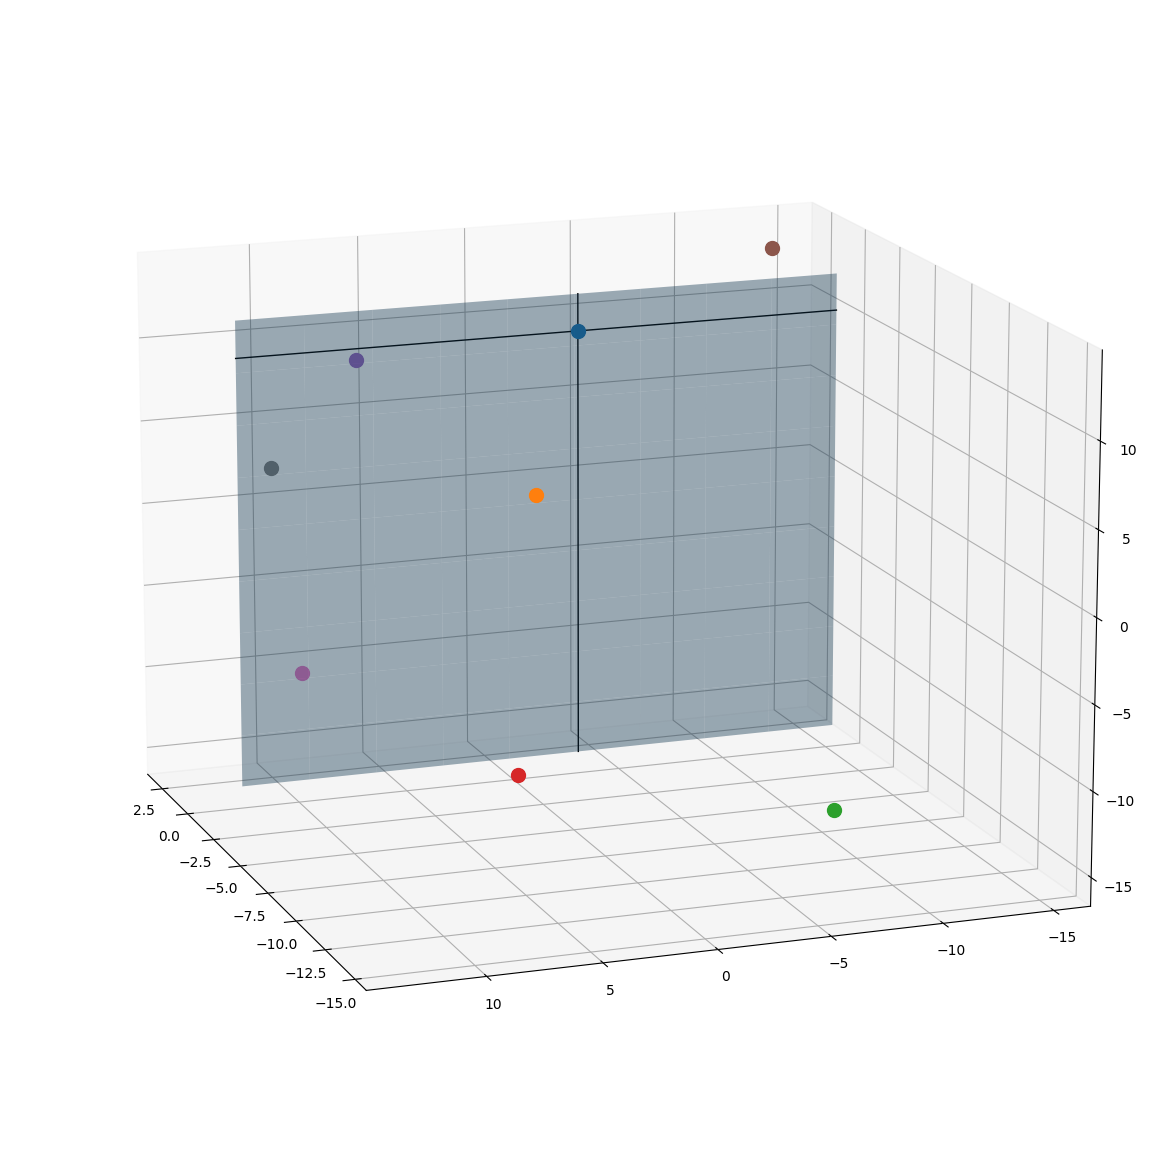
\includegraphics[width=\linewidth]{kd_tree_progress_img0.png}
            \caption{Depth 0}
        \end{subfigure}%
        \hfill
        \begin{subfigure}{.4\textwidth}
            \centering
            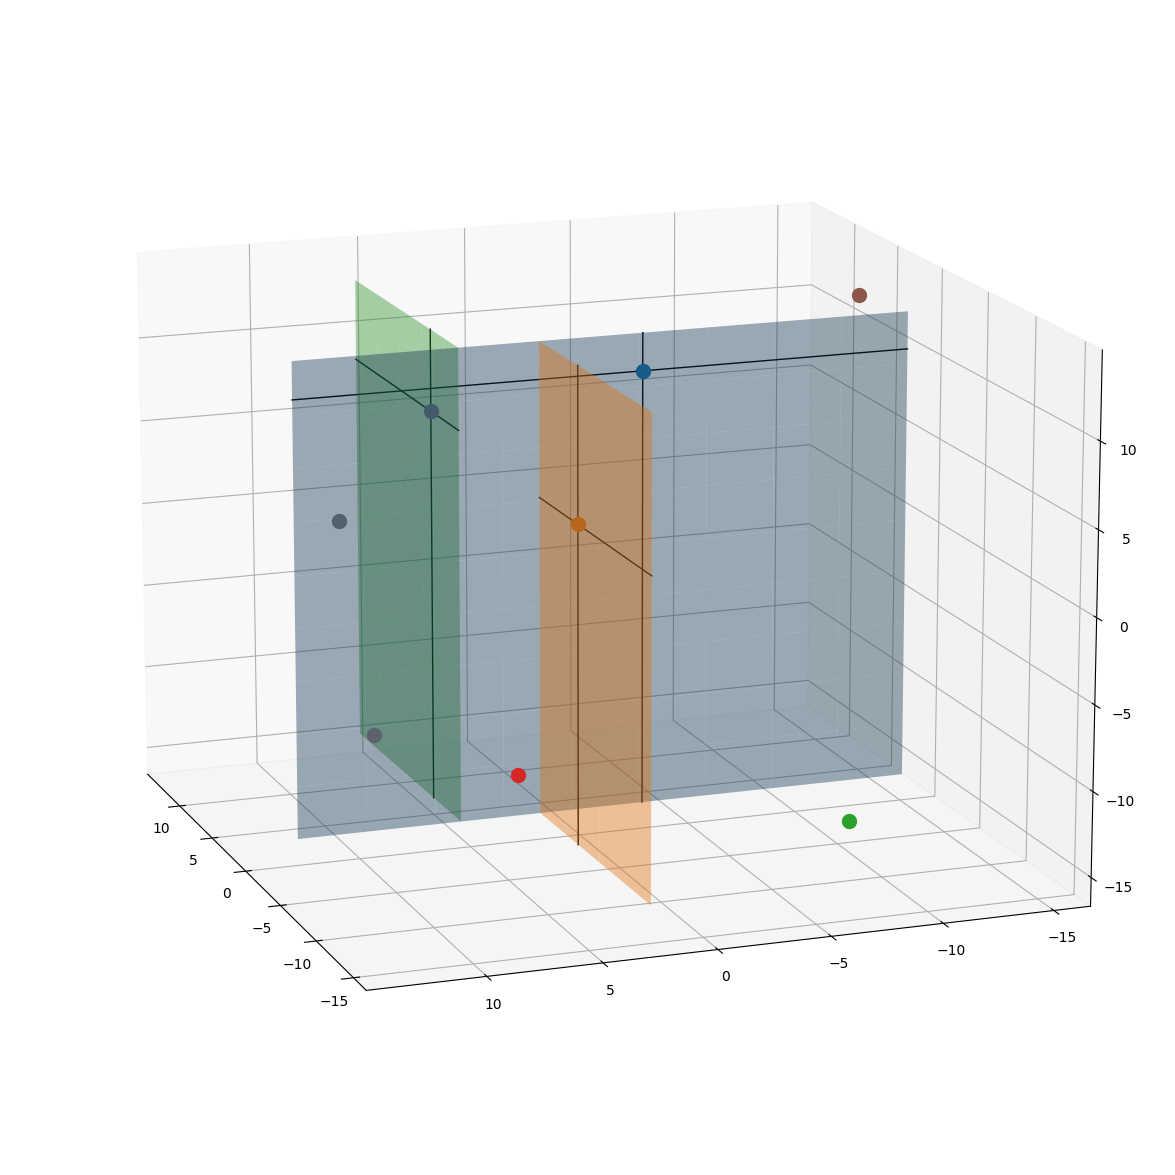
\includegraphics[width=\linewidth]{kd_tree_progress_img1.png}
            \caption{Depth 1}
        \end{subfigure}
        \hfill
        \begin{subfigure}{.4\textwidth}
            \centering
            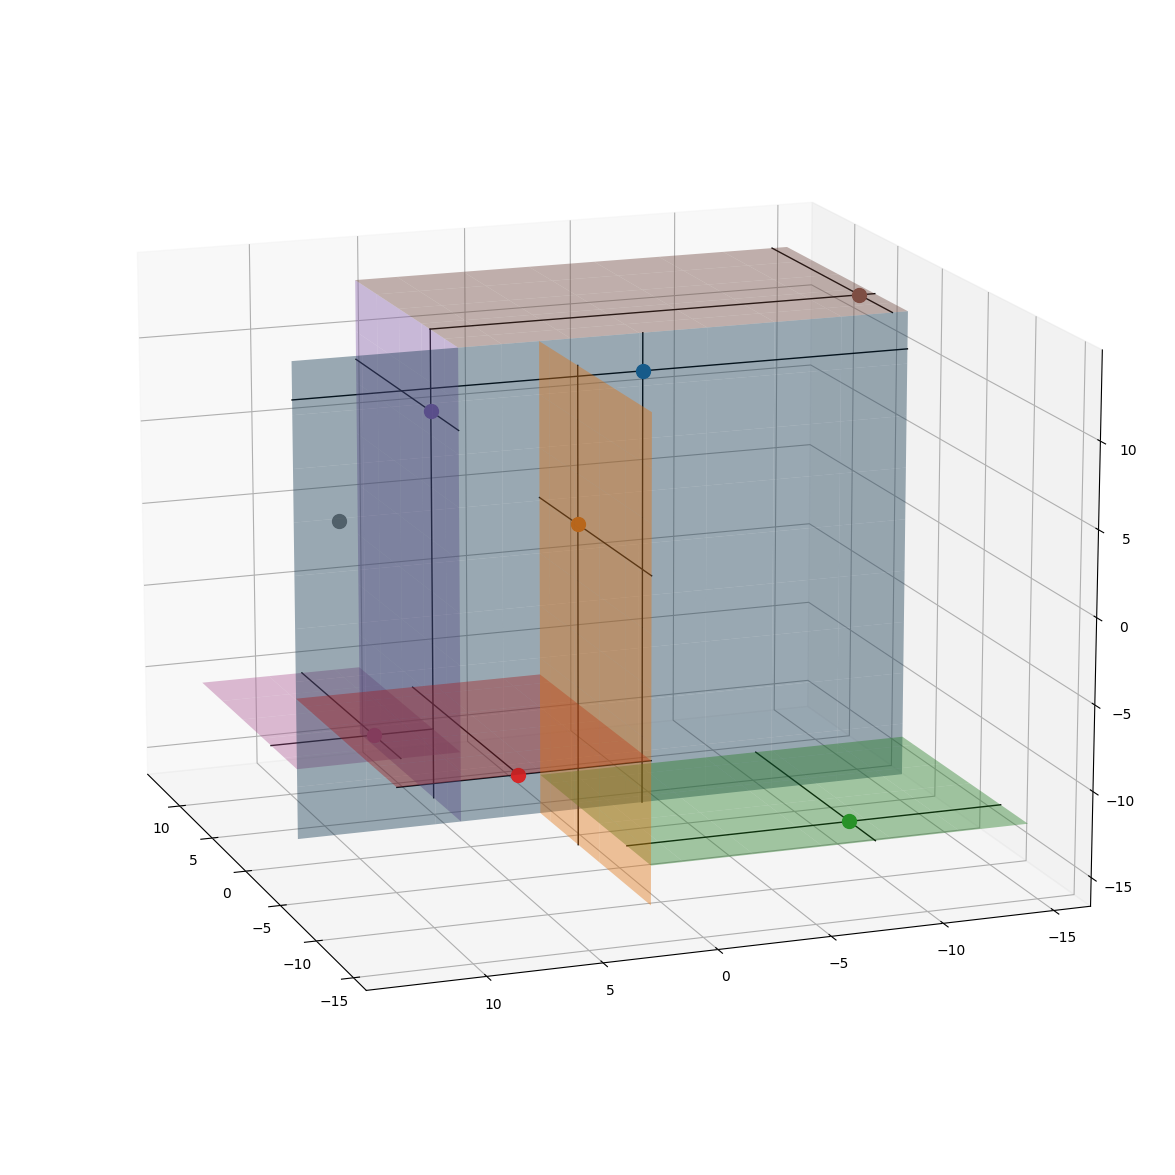
\includegraphics[width=\linewidth]{kd_tree_progress_img2.png}
            \caption{Depth 2}
        \end{subfigure}
    }
    \caption{A \kdtree{} (surfaces representation).}
    \label{fig:kdtree_surfaces_progression}
\end{figure}

The visualization in Figure \ref{fig:kdtree_surfaces_progression} renders in a
very clear way the fact that points added to the tree in the level $k$ need to
satisfy constraints given by all the points in the parent branches in levels
$0, \dots, k-1$. Each surface is the plane containing one of the points
added to the tree in the current level, which divides the volume dedicated to
the corresponding branch in two halves which shall contain all the other points
(respectively) in the left and right branch. This is almost a visual
transposition of (\ref*{eq:recursive_kdtree_definition}).

However, in order to communicate the structure of the tree
the visualization shown in Figure \ref{fig:kdtree_branches_progression} may be
preferred, which is easier to interpret visually but conveys a smaller amount
of information about the structure we imposed on the dataset.

\begin{figure}[t!]
    \makebox[\textwidth][c]{
        \begin{subfigure}{.4\textwidth}
            \centering
            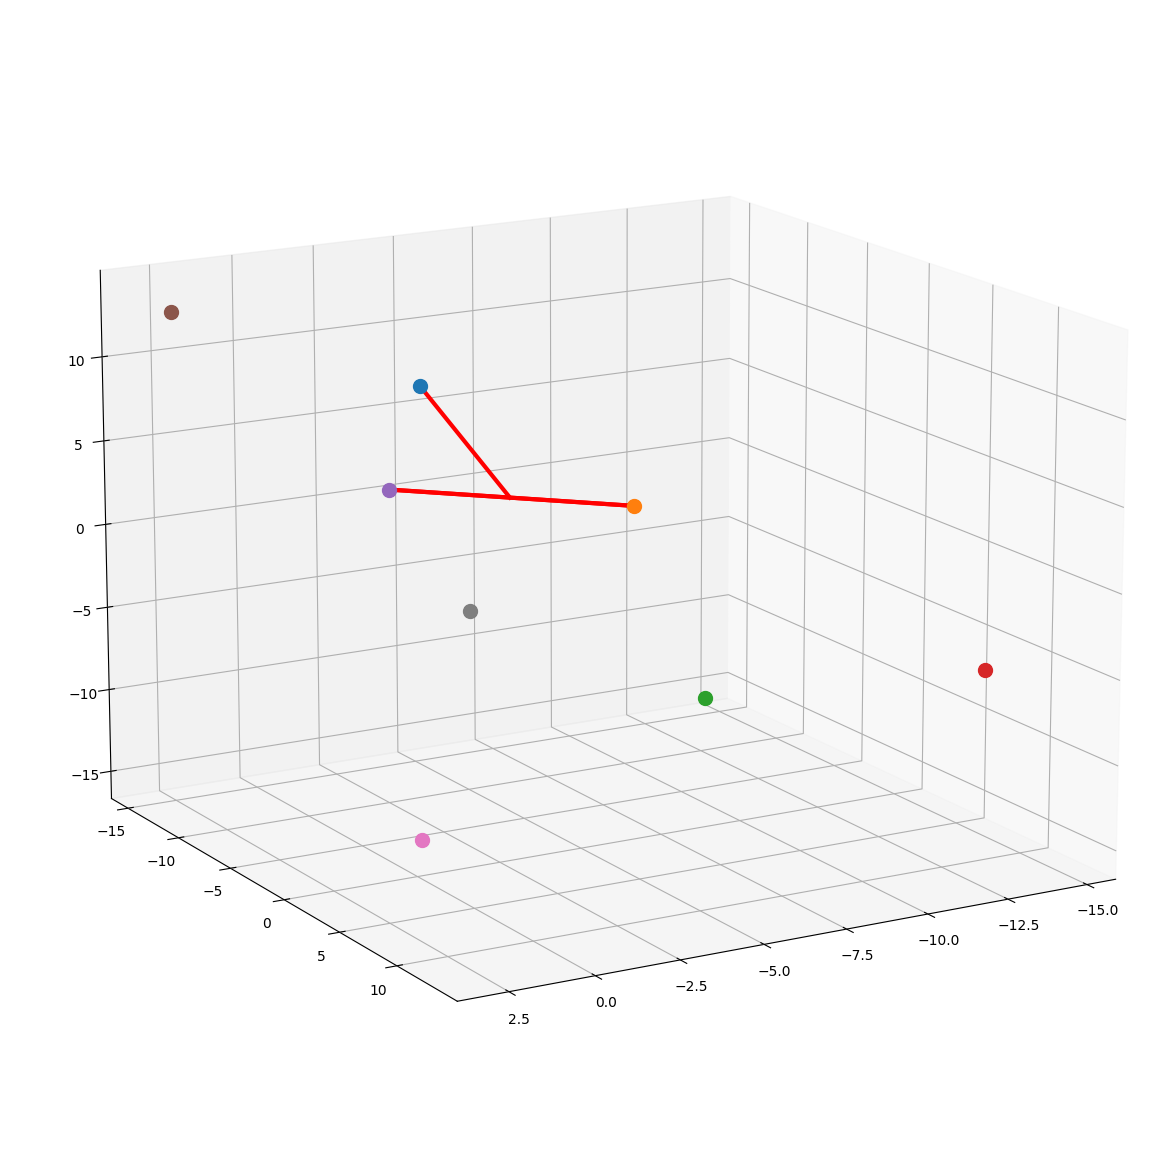
\includegraphics[width=\linewidth]{kd_tree_progress_img0_branches.png}
            \caption{Depth 0}
            \end{subfigure}%
        \hfill
        \begin{subfigure}{.4\textwidth}
            \centering
            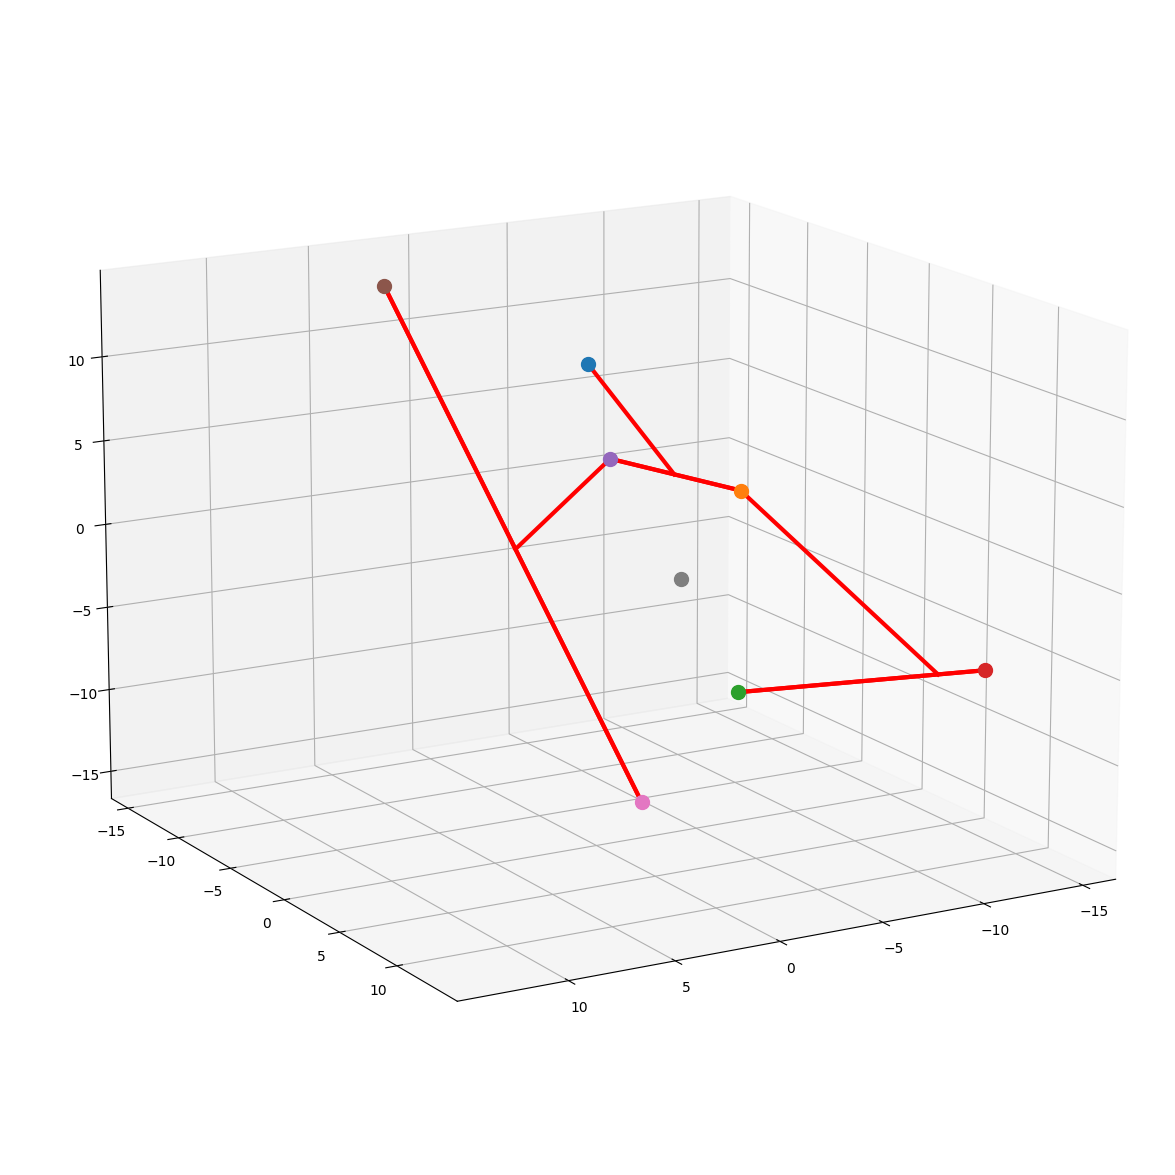
\includegraphics[width=\linewidth]{kd_tree_progress_img1_branches.png}
            \caption{Depth 1}
            \end{subfigure}
        \hfill
        \begin{subfigure}{.4\textwidth}
            \centering
            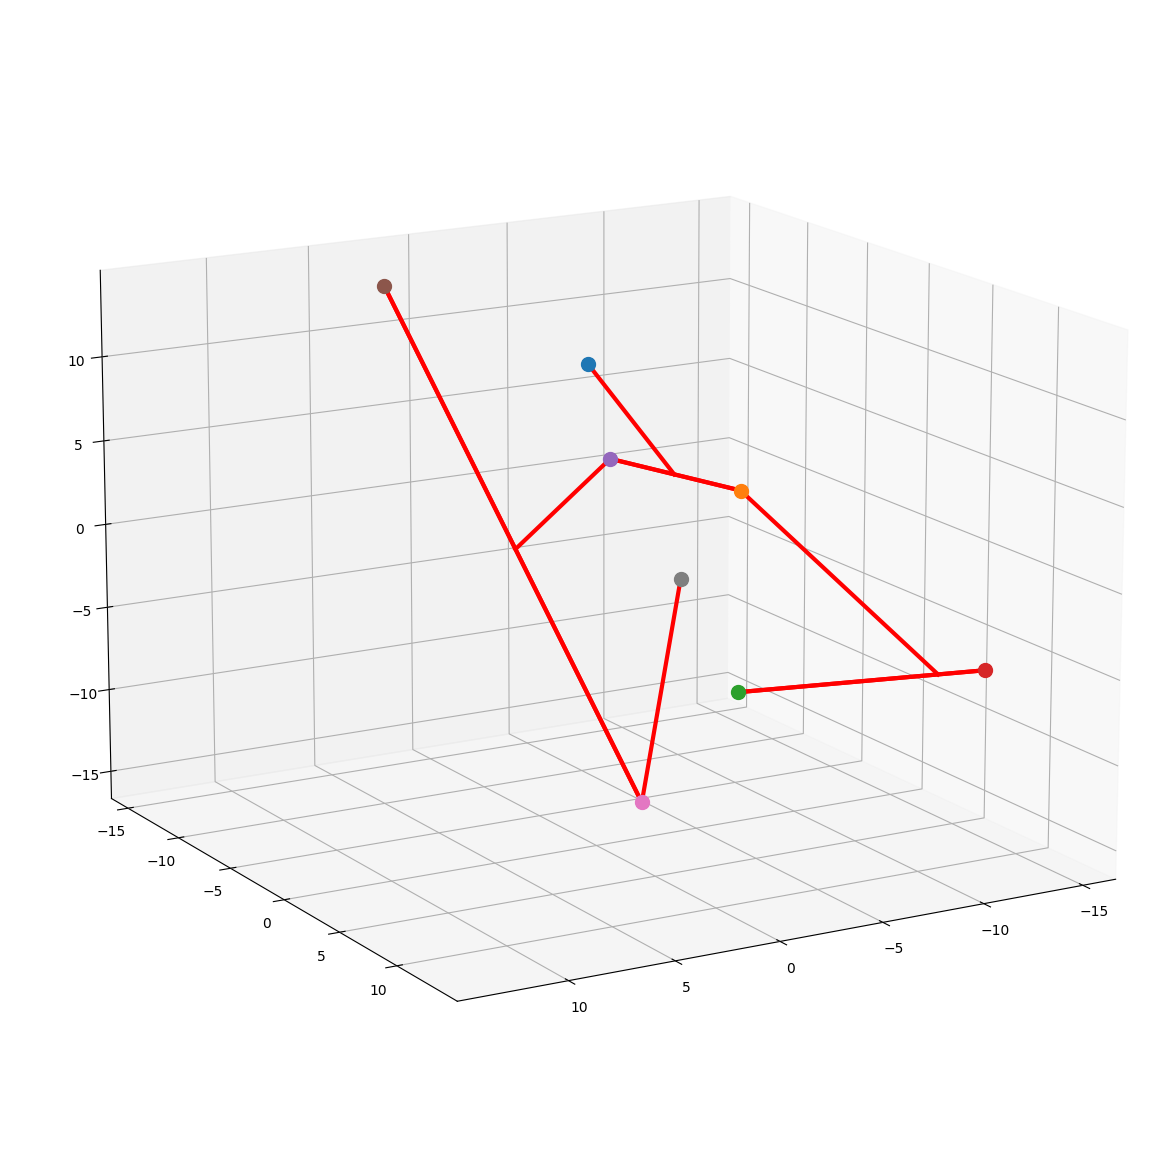
\includegraphics[width=\linewidth]{kd_tree_progress_img2_branches.png}
            \caption{Depth 2}
        \end{subfigure}
    }
    \caption{The same \kdtree{} shown in Figure \ref{fig:kdtree_surfaces_progression} (branches representation).}
    \label{fig:kdtree_branches_progression}
\end{figure}

\section{Parallel algorithm and implementation} \label{sec:algorithm}
First of all we briefly describe the parallel algorithm; then we procede
with some words and motivations regarding how we represented the dataset in our
code and which data structures we used.

The algorithm is a very simple codification of the definition proposed in
Section \ref{sec:intro}:
\begin{algorithm}
    \SetAlgoLined
    \caption{An algorithm with caption}\label{alg:parallel_algorithm}
    \KwData{$P = \{p_1, \dots, p_n\}, \ell$}
    $i \gets i(\ell)$ like in (\ref{eq:axis_criteria})\; \label{alg:first}
    Find the median point $p_m$ against the axis $i$\;
    Assign the right branch (i.e. $P_2$) to another parallel worker (if available)\;
    $P = P_1, \ell = \ell + 1$\;
    Go back to Line \ref{alg:first}\;
\end{algorithm}

The "parallel worker" exists in different instances, which depend on the
parallel framework used to run the code:
\begin{itemize}
    \item If MPI is used, a parallel worker is one of the processes employed to run the code;
    \item If OpenMP is used, a parallel worker is an OMP thread.
\end{itemize}

It's worth noting that these kind of resources are not unlimited: in case no
parallel workers are available we procede in a serial way, with two recursive
calls on the function which we use to generate the \kdtree{} for both the left
and right branch. This kind of setting requires a more refined approach if
MPI is used (OpenMP is quite convenient in this case), and we will now spend
some words on this.

Whenever we want to communicate something from an MPI process to another, we
need to know precisely what we want to send and what's the thread
(i.e. the rank) we want to communicate with. Since in principle we are going to
have multiple processes which want to communicate with multiple children
processes, we needed some way to determine the objective rank of a process
willing to take on a branch of the two branches originating from the set of
points processed by the current process. Two ideas emerged, which we present
briefly. The first one is a \emph{master-slave}  approach, i.e. to dedicate a
process to the sole work of load-balancing the computation between all the
available parallel workers. A process willing to delegate its right branch to
another MPI process would have needed to:
\begin{enumerate}
    \item Establish a communication with the \emph{master};
    \item Receive the rank of a free MPI process;
    \item Establish a communication with the chosen MPI process;
    \item Send $P_2$;
\end{enumerate}

We had the feeling that this kind of setting would have incremented by 2 units
the number of communications needed to delegate a branch to another process;
however, the code would have been most likely very elegant and understandable.
Nonetheless we decided to pursue another approach: an ``hardcoded'' protocol.
All the parent processes know right off the bat the rank of the
child process which it needs to communicate with, since it can be computed via
some very simple arithmetic operations. The code becomes less readable, but
no-one is going to notice since we decided to hide this kind of complexity
behind a function.

We briefly describe the protocol we employed in our code with a practical
example, let's say sat we have 11 MPI processes (0 is the main one), which we
represent as follows:

\begin{figure}[H]
    \centering
    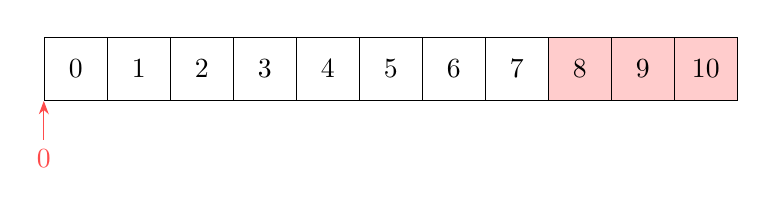
\begin{tikzpicture}
        \matrix (A) [matrix of nodes, nodes={draw, minimum size=8mm},
            column sep=-\pgflinewidth]{
            0 & 1 & 2 & 3 & 4 & 5 & 6 & 7 & |[draw,fill=red!20]|8 & |[draw,fill=red!20]|9 & |[draw,fill=red!20]|10\\};
        \foreach \i [evaluate=\i as \ni using {int(\i)}, evaluate=\i as \ntext using {int(\i-1)}] in {1}
            \draw [{Stealth}-, red!70] (A-1-\ni.south west)--++(-90:5mm) node[below] {0};
    \end{tikzpicture}
\end{figure}

The red arrow pointing to \fbox{0} means that at this point only \fbox{0} is
running, while the other MPI processes are idle, waiting for some branch to be
assigned to them. The number below the arrow refers to the current depth of the
three processed by the process that the arrow is pointing to. Also, at this
point the whole dataset is assigned to \fbox{0}. This is equivalent to
``Depth 0'' in Figure \ref{fig:kdtree_surfaces_progression} and
\ref{fig:kdtree_branches_progression}. Note that \fbox{8}, \fbox{9}, \fbox{10}
are highlighted in red. We call them \texttt{surplus\_workers} for reasons which
will be clarified in some lines.

At this point \fbox{0} executes Algorithm \ref{alg:parallel_algorithm},
which means that the left branch generated (i.e. $P_1$) is recursively assigned
to \fbox{0}. How do we choose the process that receives the right branch (i.e.
$P_2$)? We consider the set of available processes (i.e. those which are not
highlighted), we split it in two equal halves and we assign $P_2$ to the first
process of the right branch (i.e. \fbox{4}):

\begin{figure}[H]
    \centering
    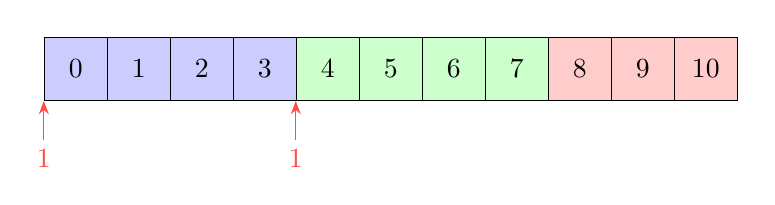
\begin{tikzpicture}
        \matrix (A) [matrix of nodes, nodes={draw, minimum size=8mm},
            column sep=-\pgflinewidth]{
                |[draw,fill=blue!20]|0 & |[draw,fill=blue!20]|1 & |[draw,fill=blue!20]|2 & |[draw,fill=blue!20]|3 & |[draw,fill=green!20]|4 & |[draw,fill=green!20]|5 & |[draw,fill=green!20]|6 & |[draw,fill=green!20]|7 & |[draw,fill=red!20]|8 & |[draw,fill=red!20]|9 & |[draw,fill=red!20]|10\\};
        \foreach \i [evaluate=\i as \ni using {int(\i)},
                        evaluate=\i as \ntext using {int(\i-1)}] in {1,5}
            \draw [{Stealth}-, red!70] (A-1-\ni.south west)--++(-90:5mm) node[below] {1};
    \end{tikzpicture}
\end{figure}

Now we have two processes working in parallel, processing two different parts of
the dataset. We keep splitting the work in the exact same way:

\begin{figure}[H]
    \centering
    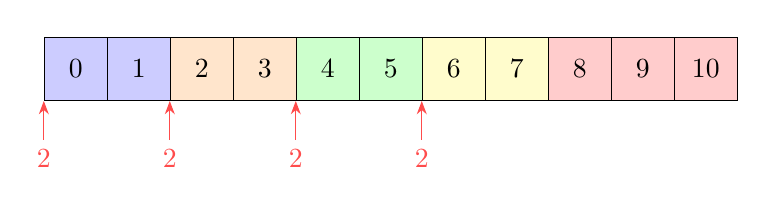
\begin{tikzpicture}
        \matrix (A) [matrix of nodes, nodes={draw, minimum size=8mm},
            column sep=-\pgflinewidth]{
                |[draw,fill=blue!20]|0 & |[draw,fill=blue!20]|1 & |[draw,fill=orange!20]|2 & |[draw,fill=orange!20]|3 & |[draw,fill=green!20]|4 & |[draw,fill=green!20]|5 & |[draw,fill=yellow!20]|6 & |[draw,fill=yellow!20]|7 & |[draw,fill=red!20]|8 & |[draw,fill=red!20]|9 & |[draw,fill=red!20]|10\\};
        \foreach \i [evaluate=\i as \ni using {int(\i)},
                        evaluate=\i as \ntext using {int(\i-1)}] in {1,3,5,7}
            \draw [{Stealth}-, red!70] (A-1-\ni.south west)--++(-90:5mm) node[below] {2};
    \end{tikzpicture}
\end{figure}

At this point we have four processes working in parallel (\fbox{0}, \fbox{2},
\fbox{4}, \fbox{6}) on the second level of the tree. Fast forward, we reach the
following situation:

\begin{figure}[H]
    \centering
    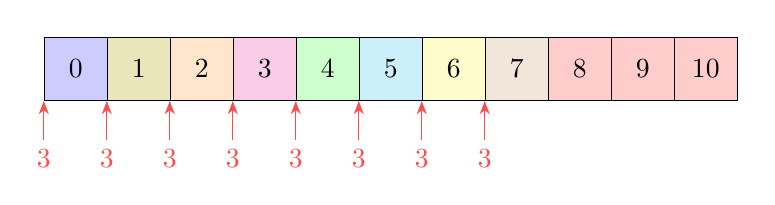
\begin{tikzpicture}
        \matrix (A) [matrix of nodes, nodes={draw, minimum size=8mm},
            column sep=-\pgflinewidth]{
                |[draw,fill=blue!20]|0 & |[draw,fill=olive!20]|1 & |[draw,fill=orange!20]|2 & |[draw,fill=magenta!20]|3 & |[draw,fill=green!20]|4 & |[draw,fill=cyan!20]|5 & |[draw,fill=yellow!20]|6 & |[draw,fill=brown!20]|7 & |[draw,fill=red!20]|8 & |[draw,fill=red!20]|9 & |[draw,fill=red!20]|10\\};
        \foreach \i [evaluate=\i as \ni using {int(\i)},
                        evaluate=\i as \ntext using {int(\i-1)}] in {1,2,3,4,5,6,7,8}
            \draw [{Stealth}-, red!70] (A-1-\ni.south west)--++(-90:5mm) node[below] {3};
    \end{tikzpicture}
\end{figure}

We now have three idle proccesses, which are clearly not enough to parallelize
entirely a new level. Even though the performance gain we get by using also
these \texttt{surplus\_workers} (we have to wait the slowest parts of the
tree to be completed) we decided to assign them left-to-right to the other
processes. In this case only \fbox{0}, \fbox{1} and \fbox{2} would get a
\texttt{surplus\_workers} (respectively \fbox{8}, \fbox{9} and \fbox{10}).
Therefore the final situation is:

\begin{figure}[H]
    \centering
    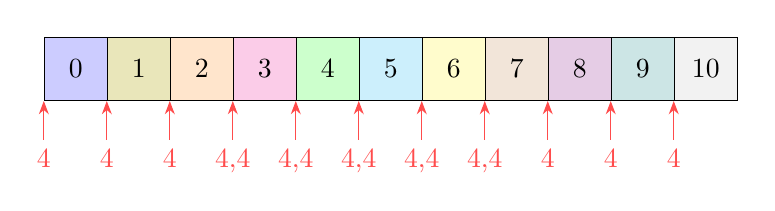
\begin{tikzpicture}
        \matrix (A) [matrix of nodes, nodes={draw, minimum size=8mm},
            column sep=-\pgflinewidth]{
                |[draw,fill=blue!20]|0 & |[draw,fill=olive!20]|1 & |[draw,fill=orange!20]|2 & |[draw,fill=magenta!20]|3 & |[draw,fill=green!20]|4 & |[draw,fill=cyan!20]|5 & |[draw,fill=yellow!20]|6 & |[draw,fill=brown!20]|7 & |[draw,fill=violet!20]|8 & |[draw,fill=teal!20]|9 & |[draw,fill=lightgray!20]|10\\};
        \foreach \i [evaluate=\i as \ni using {int(\i)},
                        evaluate=\i as \ntext using {int(\i-1)}] in {1,2,3,9,10,11}
            \draw [{Stealth}-, red!70] (A-1-\ni.south west)--++(-90:5mm) node[below] {4};
        \foreach \i [evaluate=\i as \ni using {int(\i)},
            evaluate=\i as \ntext using {int(\i-1)}] in {4,5,6,7,8}
            \draw [{Stealth}-, red!70] (A-1-\ni.south west)--++(-90:5mm) node[below] {4,4};
    \end{tikzpicture}
\end{figure}

As you can see \fbox{3}, \fbox{4}, \fbox{5}, \fbox{6}, \fbox{7} receive both the
branches they spawned, while the other processes receive only one. From now on
we do not have other MPI processes, therefore the computation proceeds serially.

As we mentioned earlier OpenMP does not requires these technicalities since we
employed OpenMP \emph{Tasks} to parallelize the computation. Everytime we need
to assign a branch to another thread we just spawn a new task, and then process
the remaining branch on this thread. We employed the modifier \texttt{final}
to disable spawning new tasks when we know that no more threads are available
since this would have stallen those tasks until a new thread is available; also
spawning OpenMP tasks without control usually leads to worse performance due the
incremented orchestration work \cite{hager2010introduction}. Checking whether
new threads are available is done almost in the same way we presented above
(even though we do not need to compute the rank of the next threads). The same
mechanism of \texttt{surplus\_workers} is employed to overcome the issues which
emerges when the number of parallel workers is not exactly the sum of consecutive
powers of 2 starting from 1.

\section{Performance model and results}

\section{Conclusions}

\bibliography{bibfile}

\end{document}
